\documentclass{beamer}

\mode<presentation> {
  \usetheme{CambridgeUS}
  \setbeamertemplate{footline}[page number]
  \setbeamertemplate{navigation symbols}{}
}

\usepackage{listings}
\usepackage{graphicx}
\usepackage{booktabs} % Allows the use of \toprule, \midrule and \bottomrule in tables

\lstdefinestyle{erlang}{
   language        = erlang,
   showstringspaces= false,
   breaklines      = true,
   keywordstyle    = {\bfseries},
   keywordstyle    = [2]{\color{green}},
   keywordstyle    = [3]{\color{red}},
   alsoletter      = {?, :},
   morekeywords    = {
     fun,
     begin},
   morekeywords    = [2]{
     ?FORALL,
     ?LET},
   morekeywords    = [3]{
     eqc:numtests,
     eqc:quickcheck,
     eqc_c:start,
     eqc\_statem:show\_states,
     car,
     car\_xml}
}
\lstdefinestyle{c}{
  language        = c,
  commentstyle    = \color{purple},
  keywordstyle    = \color{violet},
  showstringspaces= false
}
\lstdefinestyle{autosar}{
  breaklines      = falsaryframe           = l,
  showstringspaces= false,
  string          = [s]{``}{''},
  morestring      = [b]",
  basicstyle      = \color{red},
  keywordstyle    = \color{blue},
  commentstyle    = \color{green},
  stringstyle     = \color{green},
  moredelim       = [is][\color{cyan}]{|}{|},
  literate        = {<=}{{$\leq$}}{1} %% observe no comma
                    {>=}{{$\geq$}}{1},
  identifierstyle = \color{black},
  emph            = {
    WdgMExpiredSupervisionCycleTol,
    WdgM_MainFunction,
    WdgM_SetMode,
    WdgM_Init,
    WdgM_DeInit,
    WdgM_CheckpointReached,
    WdgM_CalculateAliveSupervision,
    WdgM_CheckLogicalSupervisedEntities
  },
  emphstyle       = {\color{cyan}},
  morekeywords    = {
    WDGM\_CORRECT,
    WDGM\_INCORRECT,
    WDGM\_GLOBAL\_STATUS\_OK,
    WDGM\_GLOBAL\_STATUS\_FAILED,
    WDGM\_GLOBAL\_STATUS\_EXPIRED,
    WDGM\_GLOBAL\_STATUS\_STOPPED,
    WDGM\_GLOBAL\_STATUS\_DEACTIVATED,
    WDGM\_LOCAL\_STATUS\_OK,
    WDGM\_LOCAL\_STATUS\_FAILED,
    WDGM\_LOCAL\_STATUS\_EXPIRED,
    WDGM\_LOCAL\_STATUS\_DEACTIVATED
  }
}
\lstset{language=c}


%------------------------------------------------
% TITLE PAGE
%------------------------------------------------

\title{Evaluation of validity of verification methods}

\author{Oskar Ingemarsson, Sebastian Weddmark Olsson}
\institute{Chalmers University of Technology, Mecel AB}
\date{\today}

\newcommand{\gloss}[1]{
\begin{frame}
  \frametitle{Glossary}
  \begin{description}
    \item [Supervised Entity]
    \item<#1->[Checkpoint]
    \item [Mode]
%    \item[-]
  \end{description}
\end{frame}
}

%================================================

\begin{document}

\begin{frame}
  \titlepage
\end{frame}

\begin{frame}
  \frametitle{Overview}
  \tableofcontents
\end{frame}

%------------------------------------------------
% PRESENTATION SLIDES
%------------------------------------------------
%================================================
\section{Before we begin}
%================================================


%================================================
\section{Introduction}
%================================================

\begin{frame}[fragile]
  \frametitle{Introduction}
  \begin{block}{Background}
    \begin{itemize}
        \item Vehicle are becoming more complex
        \item Circa 80 processes
        \item Close to hundred million lines of code
        \item More functionality
        \item Safety critical
        \item Testing are becoming even more important
        \item Testing more then half the production cost
    \end{itemize}
   \end{block}
\end{frame}

\begin{frame}[fragile]
  \frametitle{Introduction}
  \begin{block}{Objective}
    \begin{itemize}
        \item Automation of tests on modules in AUTOSAR
        \item Examine if it is possible to reach the requirements for
          a higher ASIL classification
        \item Functional Safety
    \end{itemize}
   \end{block}
  \begin{block}{Resources}
    \begin{itemize}
        \item Model based testing
        \item QuickCheck
        \item Other
    \end{itemize}
  \end{block}
\end{frame}

\gloss{1}

%================================================
\section{Watchdog Manager}
%================================================
\begin{frame}[fragile]
  \frametitle{Functions}
  \begin{block}{Getters}
    \begin{itemize}
      \item \lstinline!GetVersionInfo(VersionInfoType*)!
      \item \lstinline!GetMode(ModeType*)!
      \item \lstinline!GetLocalStatus(SupervisedEntityIdType, LocalStatusType*)!
      \item \lstinline!GetGlobalStatus(GlobalStatusType*)!
      \item \lstinline!GetFirstExpiredSEID(SupervisedEntityIdType*)!
    \end{itemize}
  \end{block}

  \begin{block}{Setters (interesting)}
    \begin{itemize}
      \item \lstinline!Init(ConfigType*)!
      \item \lstinline!DeInit()!
      \item \lstinline!PerformReset()!
      \item \lstinline!SetMode(ModeType, uint16)!
      \item \lstinline!MainFunction()!
      \item \lstinline!Checkpointreached(SupervisedEntityIdType, CheckpointIdType)!
    \end{itemize}
  \end{block}
\end{frame}

\gloss{2}

\begin{frame}
  \frametitle{Supervision functions}
  \begin{itemize}
    \item Alive supervision
    \item Deadline supervision
    \item Logical supervision
  \end{itemize}
\end{frame}

\begin{frame}
  \frametitle{Alive Supervision}
  \begin{block}{Statement}
    A checkpoint that is monitored by alive supervision, should be
    reached a number of times between each cycle.
  \end{block}
\end{frame}

\begin{frame}
  \begin{block}{Values/Variables}
    \begin{description}
      \item[Expected alive indications] (EAI), property of mode, fixed
        value from configuration
      \item[Supervision reference cycle] (SRC), property of mode, fixed value
        from configuration
      \item[Min margin] (Min), property of mode, fixed value from configuration
      \item[Max margin] (Max), property of mode, fixed value from configuration
      \item[Alive counter] (AC)
      \item[Supervision cycle] (SC)
    \end{description}
  \end{block}
\end{frame}

\begin{frame}[fragile]
  \begin{block}{The algorithm}
    \begin{lstlisting}
      if (SC Mod SRC == 0)
        // perform alive supervision
        if (-Min <= AI - EAI <= Max)
           Alive supervision is correct
        else
           Alive supervision is incorrect
    \end{lstlisting}
  \end{block}
  Performed in the MainFunction, also increments the supervision
  cycles.\\
  CheckpointReached increments the alive indications for a certain
  checkpoint.
\end{frame}

\begin{frame}
  \frametitle{Deadline Supervision}
\end{frame}

\begin{frame}
  \frametitle{Logical Supervision}
\end{frame}
%================================================
\section{Implementation}
%================================================
%------------------------------------------------
% \subsubsection{Stubs}
%------------------------------------------------


%------------------------------------------------
\subsection{Erlang implementation of AUTOSAR}
%------------------------------------------------

\begin{frame}
  \frametitle{How QuickCheck works}
  Generators, preconditions, postconditions, changes to model state.
  \begin{figure}
    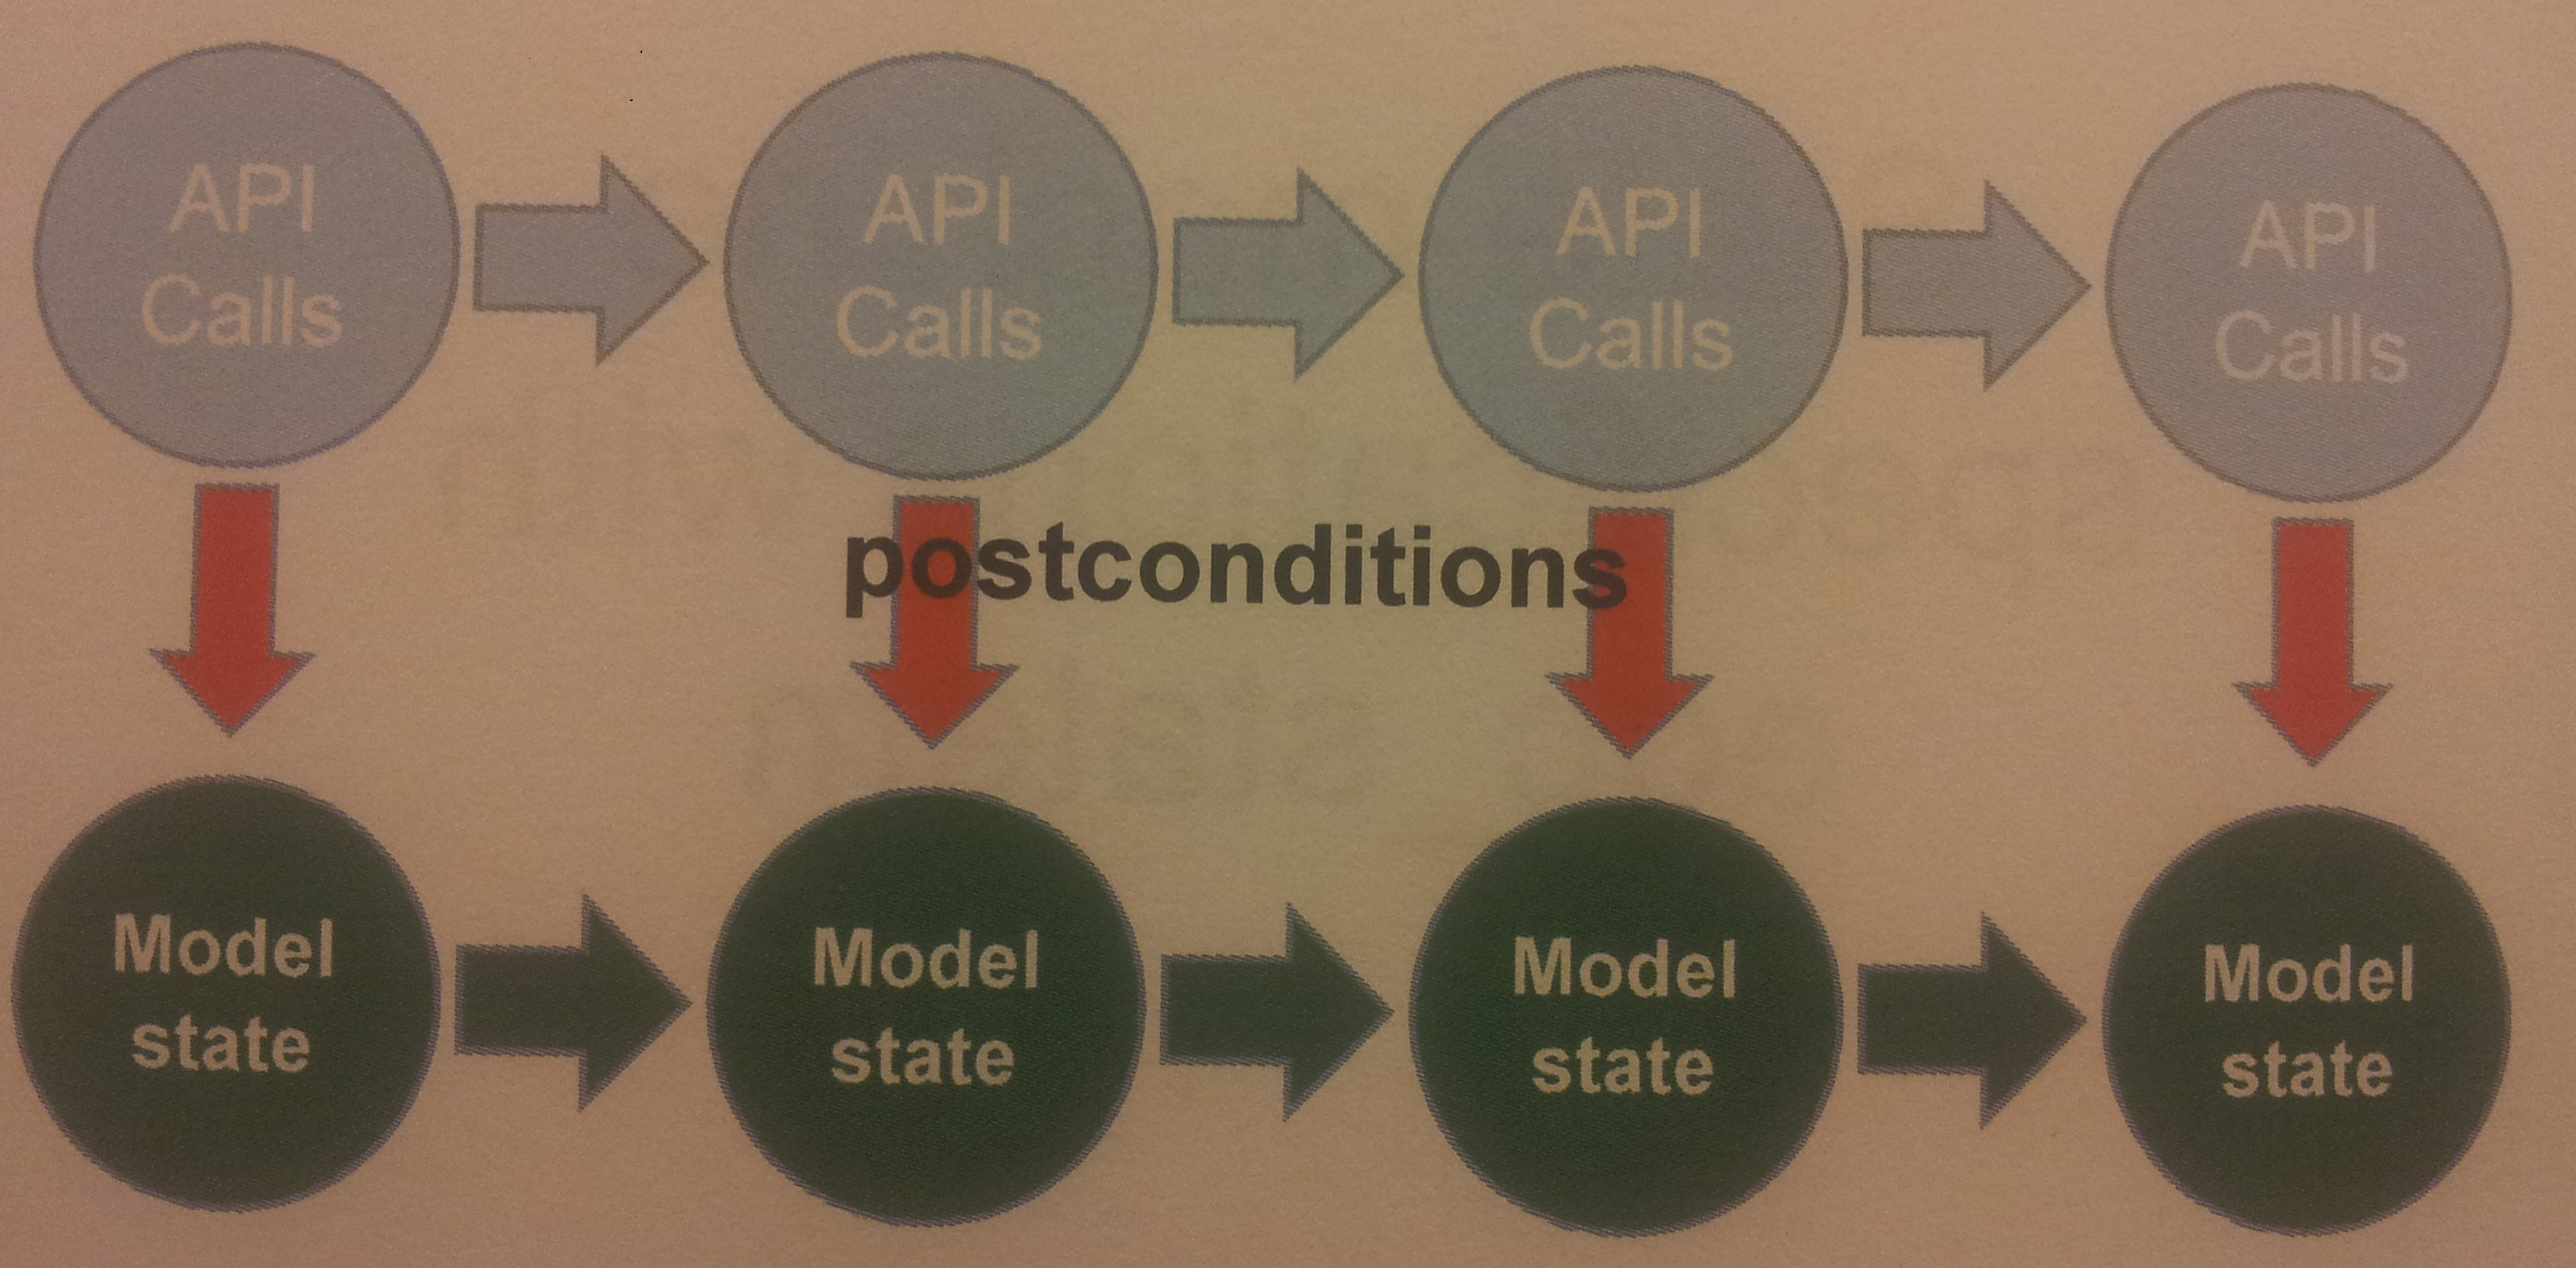
\includegraphics[keepaspectratio, width=0.7\linewidth]{api_calls}
  \end{figure}
\end{frame}

\begin{frame}
  \frametitle{Example configuration}
  Covers most of the model, still quite small.\\
  DevErrorDetect is on.\\
\end{frame}

%------------------------------------------------
\subsection{Limitations}
%------------------------------------------------

\begin{frame}
  \frametitle{DevErrorDetect}
  \begin{itemize}
    \item positive testing
    \item missing requirements
    \item segmentation faults
  \end{itemize}
\end{frame}

%----------------------------------------------
\subsection{Negative testing}
%----------------------------------------------

\begin{frame}
  \frametitle{Red}
\end{frame}

%----------------------------------------------
\subsection{Positive testing}
%----------------------------------------------

\begin{frame}
  \frametitle{Green}
\end{frame}

%------------------------------------------------
\subsection{Tweaking the generators}
%------------------------------------------------

\begin{frame}
  \frametitle{What test cases are interesting?}
  \begin{itemize}
    \item Negative testing
    \begin{itemize}
      \item good to cover bad arguments
    \end{itemize}
    \item Positive testing
    \begin{itemize}
      \item no absorbing state
      \item correct arguments
      \item correct command sequences
    \end{itemize}
  \end{itemize}
\end{frame}

\begin{frame}
  \begin{figure}
    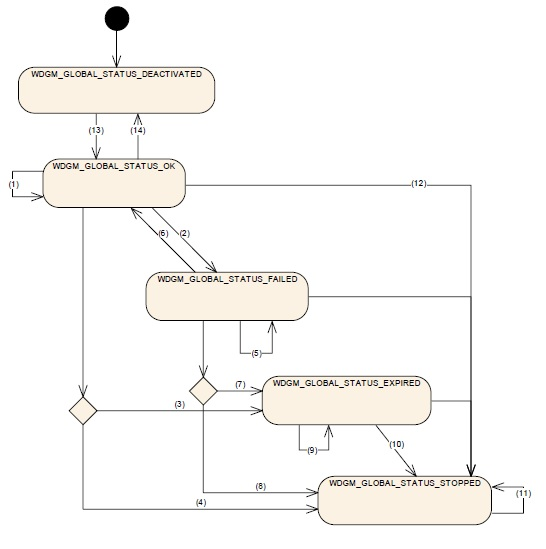
\includegraphics[keepaspectratio, width=0.7\linewidth]{globalstatuses}
  \end{figure}
\end{frame}

%================================================
\section{How to handle bugs}
%================================================
%------------------------------------------------
%\subsection{Less good methods}
%------------------------------------------------

\begin{frame}
  \frametitle{Less good methods}
  \begin{block}{Report bug}
    \begin{description}
      \item[+] Not our job to correct the code
      \item[-] Unknown time delay, probably weeks...
    \end{description}
  \end{block}

  \begin{block}{Skip the function with the bug}
    \begin{description}
      \item[+] We can continue testing
      \item[-] After finding some bugs, we don't have anything to test at all
    \end{description}
  \end{block}
\end{frame}

%------------------------------------------------
%\subsection{Good Methods}
%------------------------------------------------

\begin{frame}
  \frametitle{Good methods}
  \begin{block}{Fix Model}
    \begin{description}
      \item[+] We can continue testing
      \item[-] Cant test c-code from another configuration or updated version etc.
    \end{description}
  \end{block}

  \begin{block}{Fix C-code}
    \begin{description}
      \item[+] We can continue testing
      \item[-] Need to get knowledge of the structure etc.
    \end{description}
  \end{block}

  \begin{block}{Mocking}
    \begin{description}
      \item[+] We can continue testing
      \item[-] Need to make a model for how it should work. The pitfall is if we
        implement the mocked function after the state machine.
    \end{description}
  \end{block}
\end{frame}

%================================================
\section{The bugs have we found}
%================================================
%------------------------------------------------
%\subsection{C-code}
%------------------------------------------------

\begin{frame}
  \frametitle{C-code}
  \begin{tabular}{l l}
    Requirement & Our classification\\\hline
    WDGM286 & Medium\\
    WDGM077 & Low-Medium\footnote{\label{footnot:ett} Together their classification is Medium-High}\\
    WDGM117 & Low-Medium$^{\ref{footnot:ett}}$ \\
    WDGM215 & Low-Medium$^{\ref{footnot:ett}}$ \\
    WDGM216 & Low-Medium$^{\ref{footnot:ett}}$ \\
    WDGM219 & Low-Medium$^{\ref{footnot:ett}}$ \\
    WDGM220 & Low-Medium$^{\ref{footnot:ett}}$ \\
    WDGM182 & High\\
    7.2.3.2 & Medium\footnote{\label{footnot:tva} Together with WDGM252 and WDGM274
      this could be dangerous}\\
    WDGM255 & Low\\
    fig. 4  & Low
  \end{tabular}
\end{frame}

%------------------------------------------------
%\subsection{Generated C-code}
%------------------------------------------------

\begin{frame}
  \frametitle{Generated C-code and include-files}
  \begin{tabular}{l l}
    Requirement & Our classification\\\hline
    p. 27       & Low\\
    fig. 4      & Low\\
  \end{tabular}
\end{frame}

%------------------------------------------------
%\subsection{AUTOSAR}
%------------------------------------------------

\begin{frame}
  \frametitle{AUTOSAR}
  AUTOSAR complications
  \begin{itemize}
    \item ambiguous meaning
    \item conflicting requirements
    \item omitted requirements/explanations
    \item spelling of configuration parameters
    \item references
  \end{itemize}
\end{frame}

%================================================
\section{Testing}
%================================================
%------------------------------------------------
%\subsection{Coverage}
%------------------------------------------------

\begin{frame}
  \frametitle{Coverage}
  % if our model behave like the c model, then we can test our models function
  % coverage and check that we test all functions.
  \begin{itemize}
    \item line coverage analysis (not absolute, due to bugs in C-code)
    \item variables in the state
    \item call coverage (not absolute)
  \end{itemize}
\end{frame}

%------------------------------------------------
%\subsection{Statistics}
%------------------------------------------------

\begin{frame}[fragile]
  \frametitle{Statistics}
  \begin{itemize}
    \item generated command sequences of up to 120 commands (really no limit)
    \item 95\% starts with the command \verb!WdgM_Init!
    \item global statuses
    %% kanske hör mer till implementationen men vi borde nämna procentsatser på
    %% globalstatusar kanske?
    % \item There is five global statuses, a functional system initiates to
    %   \verb!WDGM_GLOBAL_STATUS_DEACTIVATED!, and if the command
    %   \verb!WdgM_Init! is successfully called, the global status should be
    %   \verb!WDGM_GLOBAL_STATUS_OK!. After that, only the commands
    %   \verb!WdgM_Mainfunction! and \verb!WdgM_DeInit! can change the global
    %   status.
  \end{itemize}
\end{frame}

\begin{frame}
  \begin{figure}
    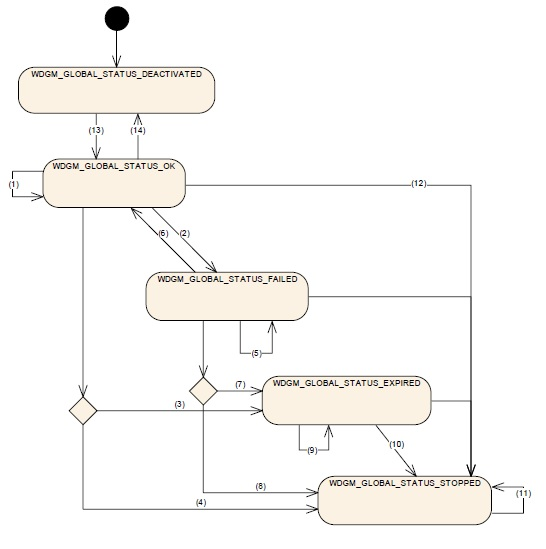
\includegraphics[keepaspectratio, width=0.7\linewidth]{globalstatuses}
  \end{figure}
\end{frame}

%------------------------------------------------
%\subsection{Suitable tests}
%------------------------------------------------

\begin{frame}[fragile]
  \frametitle{Suitability of tests}
  We generate lists of commands, most of which starts with
  \verb!WdgM_Init! or it has \verb!WdgM_Init! in the first 2-4
  commands. This is a precondition for all other functions except
  \verb!WdgM_GetFirstExpiredSEId!.\\[0.5cm]

  The functions that change the state considerably is
  \verb!WdgM_Checkpointreached!, \verb!WdgM_SetMode! and
  \verb!WdgM_Mainfunction!.  Therefor we prioritize these functions in
  the generation.
\end{frame}

%================================================
\section{Future work}
%================================================

\begin{frame}[fragile]
  \frametitle{Functional Safety}
  We will look at how this testing suites ISO26262. We have good hopes of
  achieving some kind of classification.\\[0.5cm]

  When the configuration flag \verb!DevErrorDetect! is off, you may get
  segmentation faults.
\end{frame}

\begin{frame}
  \frametitle{Bug report}
  As stated, we have found a lot of bugs and we have modified the C-code.
\end{frame}

\begin{frame}
  \frametitle{Shrinking....}
  We found out that there is some problems when QuickCheck tries to
  shrink failed tests. This is because most of the commands we send in
  depend on the state, and QuickCheck just tries to shrink the generated
  commands/arguments. Many of which will fail because some other
  (previous) command has been neglected.\\[0.5cm]

  It is possible to guide QuickCheck to shrink correctly, but it wont
  be a part of this thesis, because time.
\end{frame}

\begin{frame}[fragile]
  \frametitle{Combining modules}
  Another part of future work could be to implement a model for
  \verb!WdgIf! and get the two modules to work coherently.
\end{frame}
%------------------------------------------------

% \begin{frame}
%   \frametitle{Kolumner}
%   \begin{columns}[c]
%     \column{.45\textwidth}
%     vänster
%     \column{.5\textwidth}
%     höger
%   \end{columns}
% \end{frame}

% \begin{frame}[fragile] % Need to use the fragile option when verbatim is used in the slide
%   \frametitle{Verbatim}
%   \begin{example}[Theorem Slide Code]
% \begin{verbatim}
% Code
% \end{verbatim}
%   \end{example}
% \end{frame}

%================================================
\section{Questions}
%================================================

\begin{frame}
  \Huge{\centerline{Questions?}}
\end{frame}

\end{document}
